\documentclass[conference]{IEEEtran}
\IEEEoverridecommandlockouts
% The preceding line is only needed to identify funding in the first footnote. If that is unneeded, please comment it out.

% Akash imports

% Colton imports

\usepackage{cite}
\usepackage{amsmath,amssymb,amsfonts}
\usepackage{algorithmic}
\usepackage{graphicx}
\usepackage{textcomp}
\usepackage{xcolor}
\def\BibTeX{{\rm B\kern-.05em{\sc i\kern-.025em b}\kern-.08em
    T\kern-.1667em\lower.7ex\hbox{E}\kern-.125emX}}

\graphicspath{ {./images/} }


\begin{document}

\title{ECE 7600 Final Project:
Card Detection and Identification using Image Processing
}

\author{\IEEEauthorblockN{Akash Fiech (201754892)}
\IEEEauthorblockA{\textit{MUN Computer Engineering} \\
St. John's, Canada \\
akashf@mun.ca}
\and
\IEEEauthorblockN{Colton Neal Smith (201819604)}
\IEEEauthorblockA{\textit{MUN Computer Engineering} \\
St. John's, Canada \\
cnsmith@mun.ca
}
}

\maketitle

\begin{abstract}
    A card detection and identification system using image processing was implemented. The
    application was implemented using OpenCV's native C++ framework. The implementation functioned
    well in a constrained environment, with controlled lighting and low background noise.
\end{abstract}

\begin{IEEEkeywords}
image processing, cards, OpenCV, C++
\end{IEEEkeywords}

\section{Introduction}
For the project, playing card detection and classification was chosen. Based on research of the
topic, it was determined that image processing implementations exist that use the primitives learned
in the course. Key fundamentals used include: perspective shifting, edge detection, and intensity
processing. The main resources on card identification for this project were ``Poker Vision: Playing
Cards and Chips Identification based on Image Processing'', and a YouTube video ``Playing Card
Detection Using OpenCV-Python on the Raspberry Pi 3 + PiCamera''
\cite{opencv-card-detection}\cite{poker-vision}. While these resources were thorough, deviations
were made to fit our scope. Our card detecting application is called Most Constrained Card Detector
(MCCD).

\section{Goal}
The goal of this project is to develop a single application that, given a controlled environment
with a solid background and soft lighting, accurately detects the suit and rank of all playing cards
in a top-down image that are visible, do not overlap, and are not rotated more than 45 degrees. The
application must implement a version of the card detection pipeline defined in the paper
\cite{poker-vision}.

The application output should be the original image, with contours drawn around all cards, and the
card identification estimate overlayed on the card.

To facilitate the development of such an application, target requirements for a debug user interface
were defined as follows:
\begin{itemize}
    \item Should process images from a camera live feed in real time (greater than 15 fps for a
        single card)
    \item Should process static images loaded from disk
    \item Should provide views of all pipeline stages
    \item Should allow export of all pipeline stages
\end{itemize}

\section{Prior Art}
The pipeline this project looks to implement is defined by the paper ``Poker Vision: Playing Cards
and Chips Identification based on Image Processing'' \cite{poker-vision}. To narrow the scope of the
project, the operating criteria for the implementation was defined as a subset of the design
described in the paper. In the Poker Agent paper, the camera was placed at the seat of a hexagonal
poker table. In our criteria, the camera location was specified as overhead. Also, the Poker Agent
implementation must operate correctly in the presence of a background with external contours, like a
standard poker table with surface graphics. Our implementation must operate only in front of a solid
background. Furthermore, the lighting conditions for the Poker Agent are entirely unspecified,
whereas our criteria specify the controlled, even lighting.

Considering these narrowed criteria, the pipeline proposed in the paper was analyzed and design
alterations were made where they would simplify the pipeline while not affecting its performance
under the required operating conditions. This report outlines the similarities and differences
between our design and that of P. Martins, L. P. Reis, and L Teofilo \cite{poker-vision}.

Another source drawn upon throughout implementation of this project was the YouTube video ``Playing
Card Detection Using OpenCV-Python on the Raspberry Pi 3 + PiCamera'' by Edje Electronics - an
OpenCV card detection implemented in Python \cite{opencv-card-detection}. Although the pipeline
design for MCCD was based solely on the ``Poker Vision'' paper and Edje Electronics' YouTube video,
this project provided inspiration for user interface elements and acted as a reference for a
practical implementation of a similar image pipeline.


\section{Pipeline Design}
The pipeline design consists of two primary operations - card extraction and feature (rank, suit)
extraction and identification, each implemented using a pipeline of elementary image processing
operations. Figure \ref{fig:pipeline}, below illustrates the overall pipeline, from source image to
rank and suit estimate. Note that rank and suit extraction are executed sequentially in the Poker
Agent, but could be parallelized with ease, so they are visually represented as such.

\begin{figure}[htbp]
\centerline{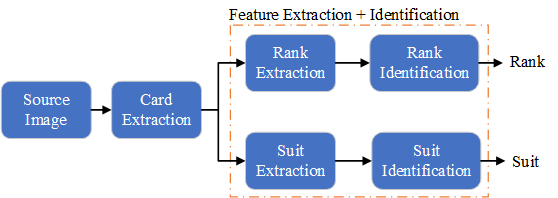
\includegraphics[width=\columnwidth]{OverallPipeline.png}}
\caption{Overall card detection and identification pipline.}
\label{fig:pipeline}
\end{figure}

\subsection{Card Extraction Pipeline}

The card extraction pipeline identifies the contour of cards in the source image and applies a
perspective transform to extract and align them. Although our criteria require operation only under
an overhead camera, applying a perspective transform offers a vehicle to align images vertically and
provides an opportunity to expand our operational capabilities with low cost and complexity.

The Poker Agent card extraction pipeline applies preprocessing to the source image, blurring it to
remove noise and applying histogram equalization to contrast stretch the image. Based on the solid
background requirement, contrast stretching will not be applied in our initial implementation. The
blurred image will be passed to a Canny Edge Detector, to extract the edges. Using these edges, the
external contours (not contained by other contours) of the image will be found. Next, the contours
will be estimated with polygons and filtered. In Poker Agent, the contours are filtered solely on
their internal angles (close to 90 are selected). Based on our constrained camera location, there is
opportunity to concisely filter the contours based on the aspect ratio of a card. As the remaining
contours represent the four corners of an image, the card can be extracted and warped to a birds eye
view using a reverse perspective transform (Figure \ref{fig:pipeline-card-extract}).

\begin{figure}[htbp]
\centerline{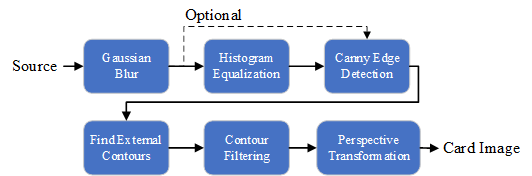
\includegraphics[width=\columnwidth]{CardExtractionActual.png}}
\caption{Card extraction pipeline.}
\label{fig:pipeline-card-extract}
\end{figure}

\subsection{Feature Extraction}
As the extraction and identification pipelines for the rank and the suit are nearly identical, they
will be referred to together. The feature image is first extracted from the card image using a
static bounding box, as the size of the cards is static and known. Although this does reduce the
likelihood of the pipeline working well with some card decks, many decks use a similar font face.
After extracting the approximate image of the feature, it is blurred and binarized with adaptive
thresholding.

In Poker Agent, the next step would be to erode to “remove remaining noise”. However, we plan to
dilate and then erode in a closing operation. The purpose of this is threefold - reconnect portions
of ranks and suites that could be separated by noise, and to connect the digits in the character ten
so they are treated as one symbol after we crop to the contour. The Poker Agent solves the 10
problem using an image wide 1-pixel wide line to artificially connect the characters (Figure
\ref{fig:pipeline-feature-extract}).

\begin{figure}[htbp]
\centerline{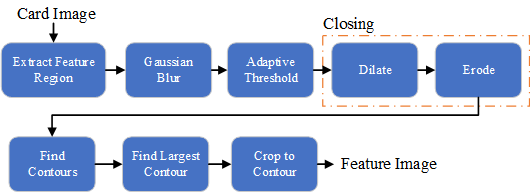
\includegraphics[width=\columnwidth]{feature-extraction.png}}
\caption{Feature extraction pipeline.}
\label{fig:pipeline-feature-extract}
\end{figure}

\subsection{Feature Identification}
To identify the feature in the image (whether it be a suit or a rank), the extracted feature image
is compared to a set of preset templates (high detail images of all ranks and suits). In Poker
Agent, template matching is used on a sprite map of ranks and suits. As our cards do not use the
same font, we will generate our own set of templates. Also, instead of template matching we will be
using a simpler approach that takes the absolute value of the difference between the feature image
and each template, then calculates the average value of the resulting mask. The mask with the lowest
average value will be produced by the two images that are most similar. The corresponding template
index / name will be the output - an estimate of what feature is being processed. The simple
“template matching” algorithm is outlined below (Figure \ref{fig:pipeline-feature-identification}).

\begin{figure}[htbp]
\centerline{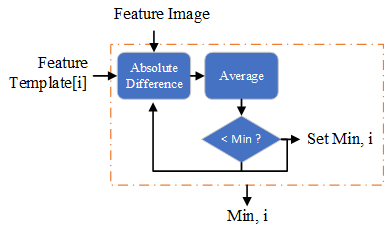
\includegraphics[width=\columnwidth]{FeatureIdentification.png}}
\caption{Feature extraction pipeline.}
\label{fig:pipeline-feature-identification}
\end{figure}

\section{Implementation}

\subsection{Language and Framework}
For this project the use of the OpenCV image processing framework with the C++ programming language
was chosen. This choice was made since OpenCV is the industry standard for image processing, it is
extremely well documented and there are multiple tutorials available. C++ was chosen because it is
the native implementation of OpenCV, is more performant than Python, and allows for lower level
optimizations when needed during the image processing program.

Along with OpenCV the OpenCV Graph API (G-API) was chosen for our image processing pipeline. Similar
to shader pipelines with game engine frameworks, the G-API allows for better modularity and
pipelining of the process. This module of OpenCV is still in its early stages and has some minor
issues, but overall the use of the G-API greatly improved development time than without.

Finally the last library used was cvui, an open source graphical user interface framework using
OpenCV. This was selected so that buttons and sliders could be used when calibrating the card
identifier and views of the intermediate stages could be seen. This greatly improved development
time as we could debug different parameters in real time.

\subsection{Interface}
The final implementation has a GUI, with a settings section, active image section, and individual
card section. In the settings section the Pipeline Stage slider changes the active image to the
specified pipeline stage. The Suit/Rank Stage slider changes the individual card view image to the
selected pipeline stage of suit/rank detection. Following those two sliders there are buttons two
save the active image and individual card view image to files. Bellow is a checkbox that toggles
between the live camera feed and the predefined image file. Finally there are multiple sliders where
one can set parameters for pipeline processes such as Kernel size for the Gaussian blur filter
(Figure \ref{fig:gui}).

\begin{figure}[htbp]
\centerline{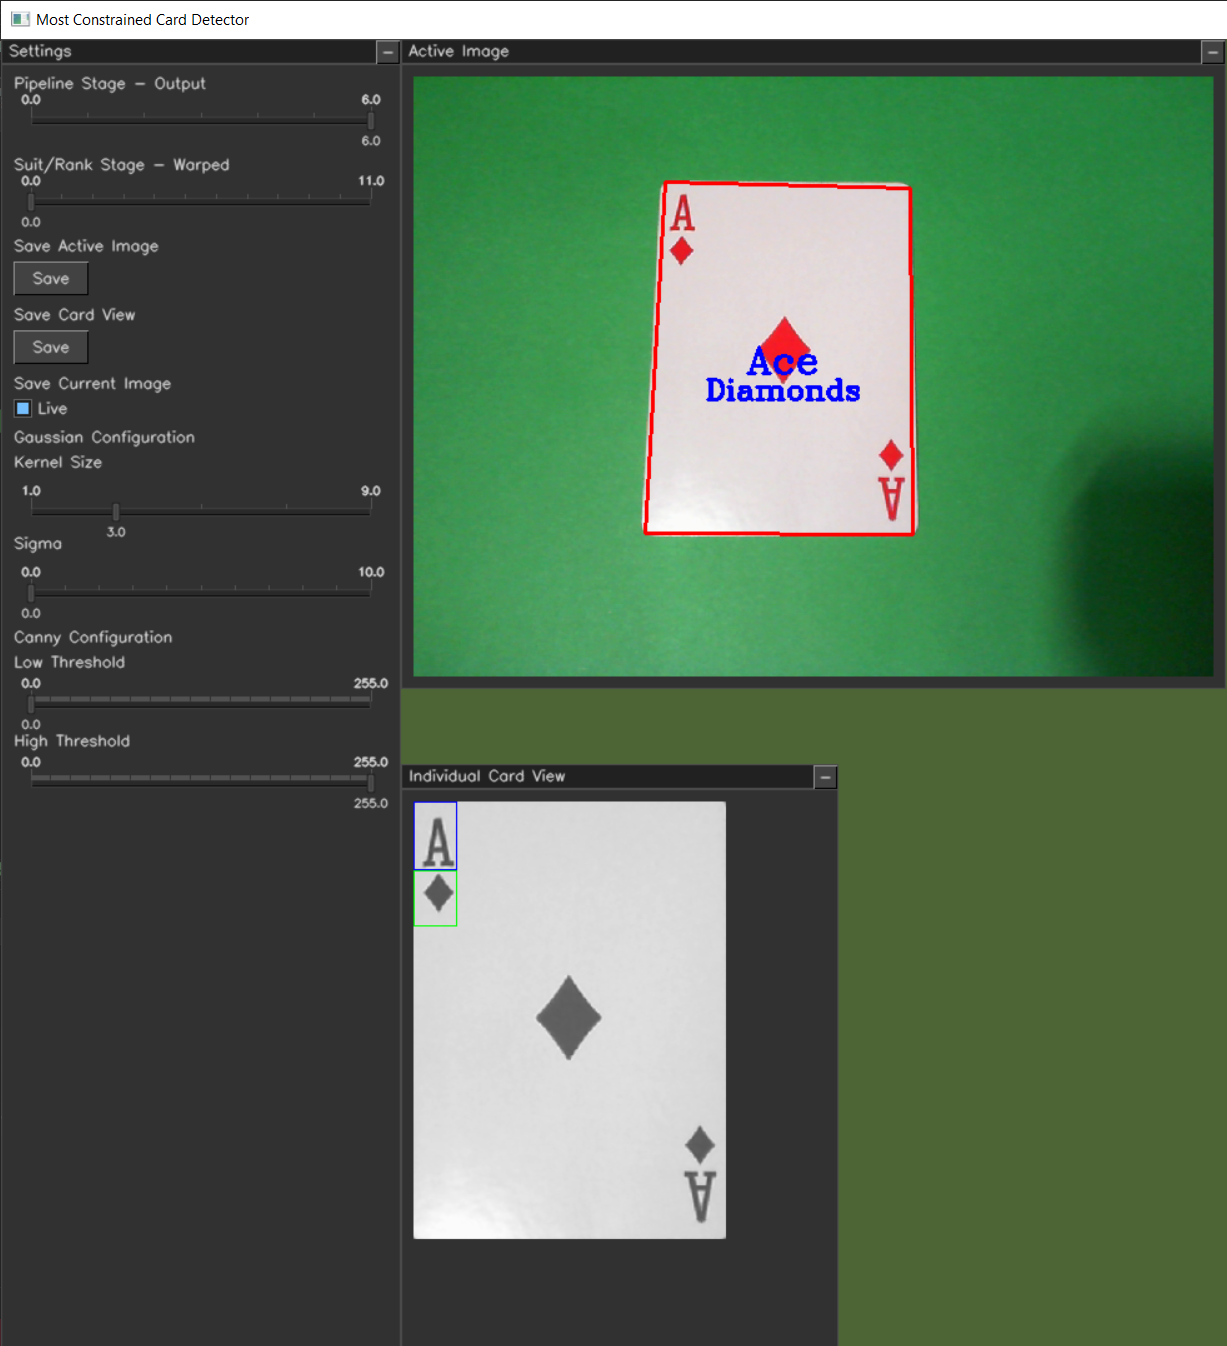
\includegraphics[width=\columnwidth]{gui.png}}
\caption{GUI for card identifier program using cvui Library.}
\label{fig:gui}
\end{figure}

\subsection{Pipeline}
In the final implementation the histogram equilization is omitted based on performance testing, under
the specified environment criteria and constraints it performed better. Figure
\ref{fig:extraction-pipeline} shows the final card extraction pipeline and the image outputs of each
stage.

\begin{figure}[htbp]
\centerline{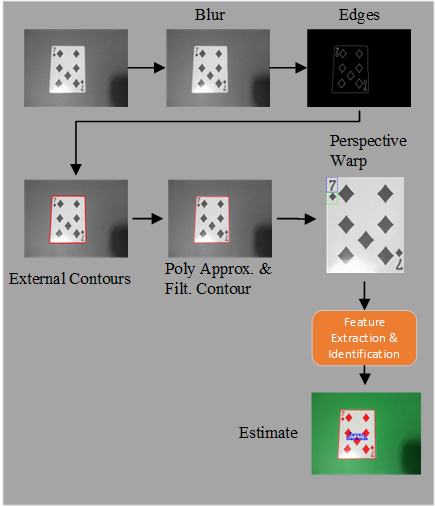
\includegraphics[width=\columnwidth]{ActualCardExtraction.png}}
\caption{Card extraction pipeline and corresponding output.}
\label{fig:extraction-pipeline}
\end{figure}

The feature extraction and identification pipeline underwent a minor change from the initial design.
Otsu's method was used in place of adaptive thresholding, in the constrained environment Otsu's
method is performant and provides comparable out to adaptive thresholding. Figure
\ref{fig:feature-extraction-pipeline} shows the final feature extraction and identification pipeline
and image output for each stage.

\begin{figure}[htbp]
\centerline{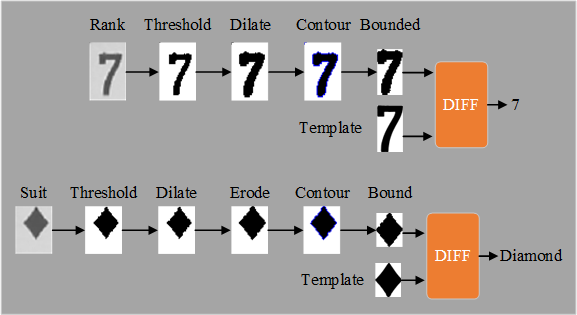
\includegraphics[width=\columnwidth]{PipelineExecFlowchart.png}}
\caption{Feature extraction and identification pipeline with corresponding output.}
\label{fig:feature-extraction-pipeline}
\end{figure}

\subsection{Encountered Issues}
Once the contours of the card are obtained it is necessary to perspective shift to a known size for
feature extraction. The corners of the card are estimated using the contours, however the points
need to be mapped to the perspective shifted image in a manor that provides the scaled image of a
card with the suit and rank information at the top left corner. The perspective shift introduced a
trade-off issue; account for all rotations at the cost of development time. A custom method was
chosen where the center of the card was found and used as the origin of a graph, and then assumed
the corner point in Quadrant 2 to be top left, point in Quadrant 1 to be top right, and so on
(Figure \ref{fig:graph}). Since the card is symmetrical about the middle of the long side, this
allows for about 180 deg of card position that will work with the model.

\begin{figure}[htbp]
\centerline{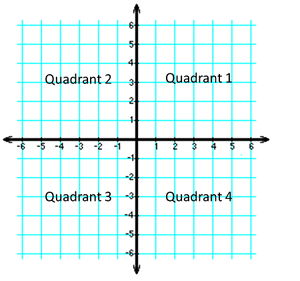
\includegraphics{graph-quadrants.png}}
\caption{Quadrants of a graph}
\label{fig:graph}
\end{figure}

The output of the preprocessed rank and suit images (identifier images) were matched against a
template image of the rank and suit that was found online. Initially this provided extremely poor
matching; therefore, images were taken of all the necessary identifiers and then by hand cropped and
thresholded into a custom identifier image (Figure \ref{fig:templates}). This greatly improved
performance for our card deck, with the downside that it is only calibrated for a single deck of
cards.

\begin{figure}[htbp]
\centerline{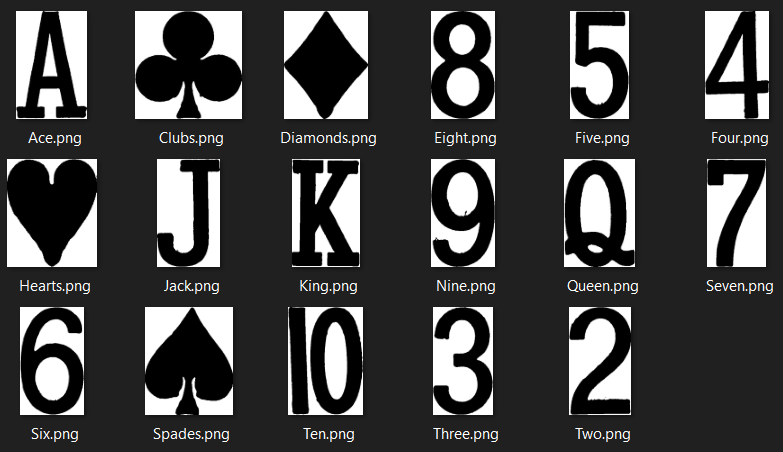
\includegraphics[width=\columnwidth]{templates.png}}
\caption{The hand made card identifier templates}
\label{fig:templates}
\end{figure}

After testing the implementation, spade face cards were being consistently misidentified as a
diamond. This was caused by the dilation of the spade suit image connecting it to the border of the
face card (Figure \ref{fig:bad-jack}).

\begin{figure}[htbp]
\centerline{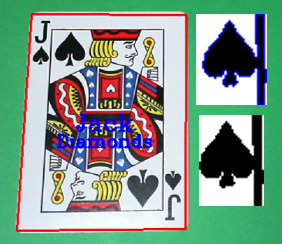
\includegraphics[width=\columnwidth]{bad-jack.png}}
\caption{Misidentified jack of spades.}
\label{fig:bad-jack}
\end{figure}

To avoid connecting these edges while maintaining the closing operation, the morphological cross was
reduced in size from 3x3 to 2x2. Figure \ref{fig:good-jack} shows the results of this improvement.

\begin{figure}[htbp]
\centerline{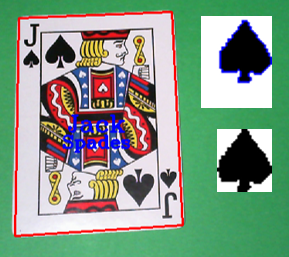
\includegraphics[width=\columnwidth]{good-jack.png}}
\caption{Misidentified jack of spades.}
\label{fig:good-jack}
\end{figure}

\section{Results}
Overall the detection of cards was very accurate in the highly constrained environment. To test the
accuracy of the implemented card detector, an entire deck of cards was tested rapidly using the live
view. The detector was able to correctly identify all cards in the deck, provided they were rotated
off axis minimally (less than 45 degrees to the left or right). A video was captured for posterity.

As the feature extraction is the most sensitive part of the pipeline, a set of feature extraction
pipeline stages was captured for confirmation of proper performance (Figure
\ref{fig:rank-extraction}.

\begin{figure}[htbp]
\centerline{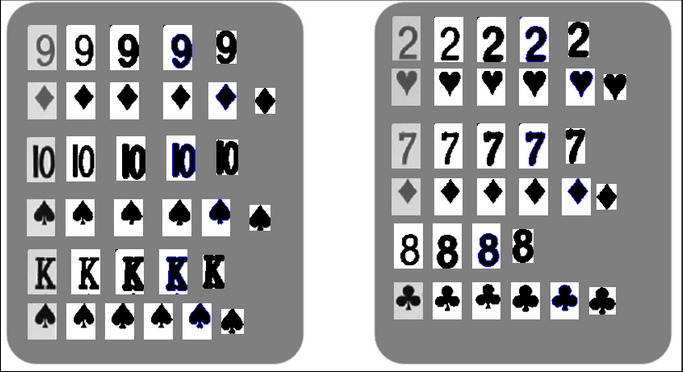
\includegraphics[width=\columnwidth]{rank-extraction.png}}
\caption{Rank extraction examples, showing pipeline stages.}
\label{fig:rank-extraction}
\end{figure}

 Multi-card performance accuracy was the same, other than lower frame rates (Figure \ref{fig:multi-card-image}).

\begin{figure}[htbp]
\centerline{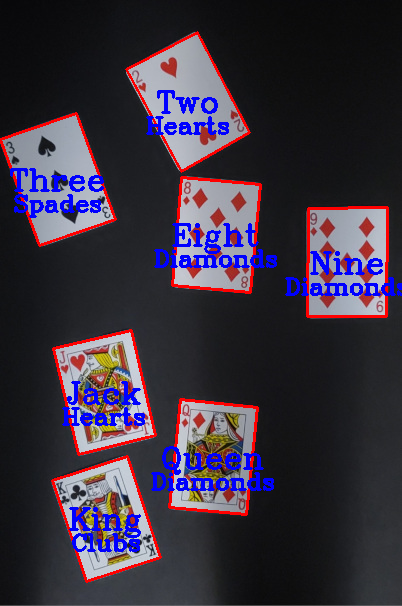
\includegraphics[width=\columnwidth]{multi-card-image.png}}
\caption{Multi-card image card example.}
\label{fig:multi-card-image}
\end{figure}


\section{Computational Performance}
The initial benchmark that we set for our programs computational performance was around 5 frames per
second (fps), this is the speed that we observed in other usable implementations (they were running
on a Raspberry Pi 3, therefore performance is expected to be lower) \cite{opencv-card-detection}.
Our implementations general speed was around 20 fps (With 7 card on screen).

\section{Limitations}
The following are limitations of the application:
\begin{itemize}
\item Calibrated to a specific card pack. Although un-tested, other card packs would likely
        experience reduced accuracy.
\item The entire card must be on the image being processed. If the card contour is broken at all
        detection will fail. This also holds true for overlapping cards; therefore, cards must not
        overlap each other (which is extremely common in card games).
\item The rotation of the card on the page must be within 45 deg from upright. The matching of the
        corners to the perspective transform is based of the position of the corner relative to the
        cards center point. Therefore an upside down card is fine due to the nature of the card
        descriptions on both top left corners. So there is about 180 deg discontinuous position
        where the detection will work.
\item Bright shining lights that reflect off the card can wash out key features that are used to
        detect the card, though it is still readable to humans.
\item Card-like objects will generate a estimate despite not being a card.
\end{itemize}

\section{Practical Applications}
Gambling is one of the most lucrative ventures on the planet - and preventing people from cheating
is likely a top priority for most gambling corporations. Yet, many card games are ``beatable'' - black
jack is a perfect example. Instead of security personnel monitoring the casino floor at all times,
card detection could be used to track player statistics, their betting patterns and winnings, to
determine whether they fit the statistical profile of a ``Cheater''.

Modern poker makes extensive use of GTO, or Game Theory Optimal strategy - an umbrella term for
poker theory founded in statistics. Bots and GTO solvers are prevalent in online poker - However
this is also a problem in live poker. In online poker, player behavioral patterns can be monitored.
In live poker, this is a much harder problem to solve. If a player can communicate with an external
party with access to a solver they can cheat the house and the other players.

Using image processing to detect cards on the table and monitor player behavior, casinos could
prevent this type of cheating given a large sample size. The Poker Agent agent pipeline followed in
this implementation of card detection is focused on the application of an autonomous poker agent.
However, a more static application such as an overhead tracking camera mounted above the table is
another very practical application of this tool.

\section{Future Improvements}
While MCDC are happy with the state of our application we realize there is still place for
improvement. The potential improvements are mostly derived from the shortcomings in the
\ref{Limitations} section.

To handle full 360 degree rotation of the cards we could improve upon our corner detection by taking
into account the distance between points and then matching the card length and with, so that we
always receive the top corners as being the shorter width of the card. This would allow the
perspective transform to always map the card so that the rank and suit info is in the top left
corner.

The application is currently calibrated for a specific card pack with a specific font for the rank
and suit identifiers. To improve the versatility of the program we could generate more reference
identifiers and then determine rank and suit based upon a statistical model. With a large enough
reference bank we could probably cover a very large range of usable cards.

While we were surprised by the speed of our application (running at around 20 fps), we could
definetly improve upon the speed. Currently the base CPU implementation for OpenCV is being used for
image processing; this could be changed to use the OpenCV CUDA or OpenCV backend. This would greatly
improve speed as the amount of parallel instructions running would drastically increase.

\section{Conclusions}
The implementation of playing card detection and identification using image processing and OpenCV
was a great learning experience. We were able to test our fundamental knowledge of image processing
and learn a bit beyond what we were taught in class. Overall we are happy with the outcome of our
application; we were able to reliably detect almost all cards. There were still cases with specific
cards where the output would be consistently incorrect. Other than that the main issues with the
current implementation is that there are conditions such as cut off cards, overexposed lighting,
orientation, etc. that cause the identification of cards to fail. A couple strategies at mitigating
these issues have also been discussed along with potential to improve computational performance.

\begin{thebibliography}{00}
\bibitem{poker-vision} P. Martins, L. P. Reis, and L Teofilo, ``Poker Vision: Playing Cards and
    Chips Identification based on Image Processing''.
\bibitem{opencv-card-detection} Edje Electronics. Playing Card Detection Using OpenCV-Python on the Raspberry Pi 3 + PiCamera. (Oct. 10, 2017). Accessed: July 5, 2022. [Online Video]. Available: https://youtu.be/m-QPjO-2IkA
\end{thebibliography}
\vspace{12pt}

\end{document}
